
\newcommand{\FigCiphersuites}{
\begin{figure}[ht]
    \centering
    \includegraphics[width=0.9\linewidth,clip]{figures/selected-cdf.pdf}
    \caption{\textbf{Cipher Suite Selection CDF}\,---\, %
    CDF of cipher suites. We show the CDF of the total number of cipher suites 
    in ClientHello
    messages as a fraction of connections observed in green. For example, approximately 50\% of
    connections observed had 15 or fewer cipher suites in the ClientHello. We 
    also plot the CDF
    of the rank of the server-selected cipher suite in the corresponding 
    ClientHello list in red.
    For instance, 90\% of ServerHellos observed selected a cipher suite in the 
    top 10 of the client's
    list. The sizeable gap between rank CDF and length CDF suggests that servers are honoring client suite order when selecting an appropriate algorithm.
    }
    \label{fig:selected-cdf}
\end{figure}
}


\newcommand{\FigBrowsers}{
\begin{figure}[ht]
    \centering
    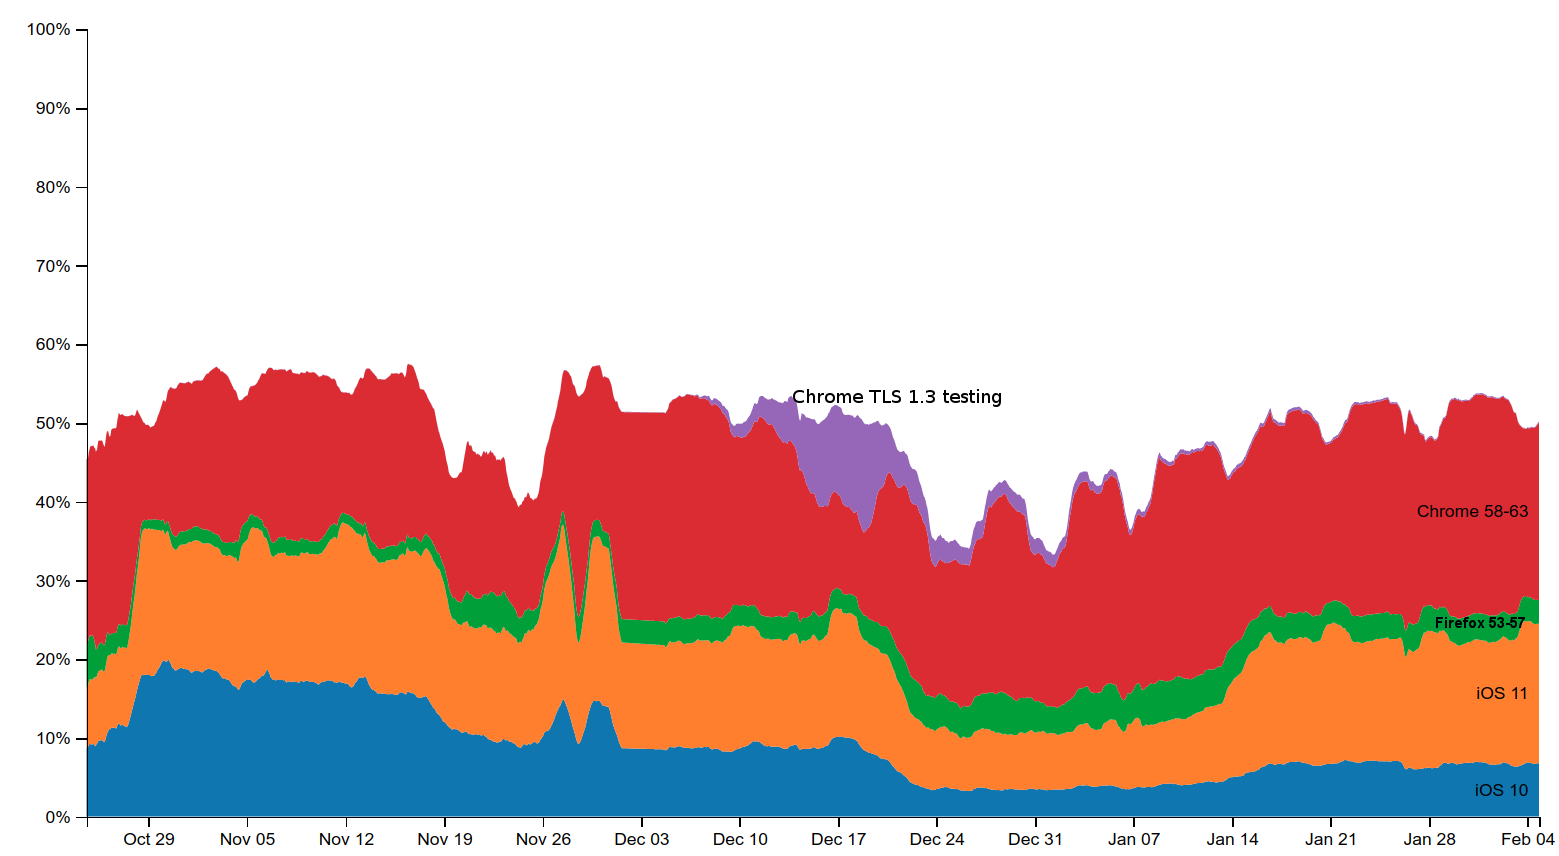
\includegraphics[width=0.9\linewidth,clip]{figures/browsers.png}
    \caption{\textbf{Popular Clients}\,---\, %
            Stacked graph showing the percent of connections (averaged over 24 hours) of popular clients,
            including recent versions of Chrome, Firefox, and versions
    of Apple iOS.  These popular clients make up roughly half of all seen connections.
    Also visible is the brief experiment Google Chrome performed in December where clients sent
    TLS~1.3 ClientHellos. 
    }
    \label{fig:browsers}
\end{figure}
}


\newcommand{\FigWhitelistChurn}{
	\begin{figure}[ht]
		\centering
		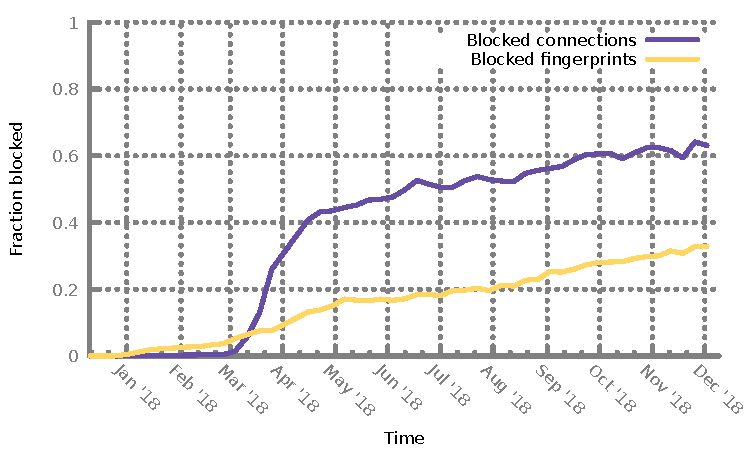
\includegraphics[width=0.9\linewidth,clip]{figures/churn.pdf}
		\caption{\textbf{Fingerprint turnover}\,---\,
            Shows fraction of connections/fingerprints not seen during the
            first week. This roughly models the fraction that censor would overblock,
            if they took a static fingerprint snapshot and whitelisted it.
        }
	\label{fig:wl-churn}
    \end{figure}
}


\newcommand{\FigTLS}{
\begin{figure}[ht]
    \centering
    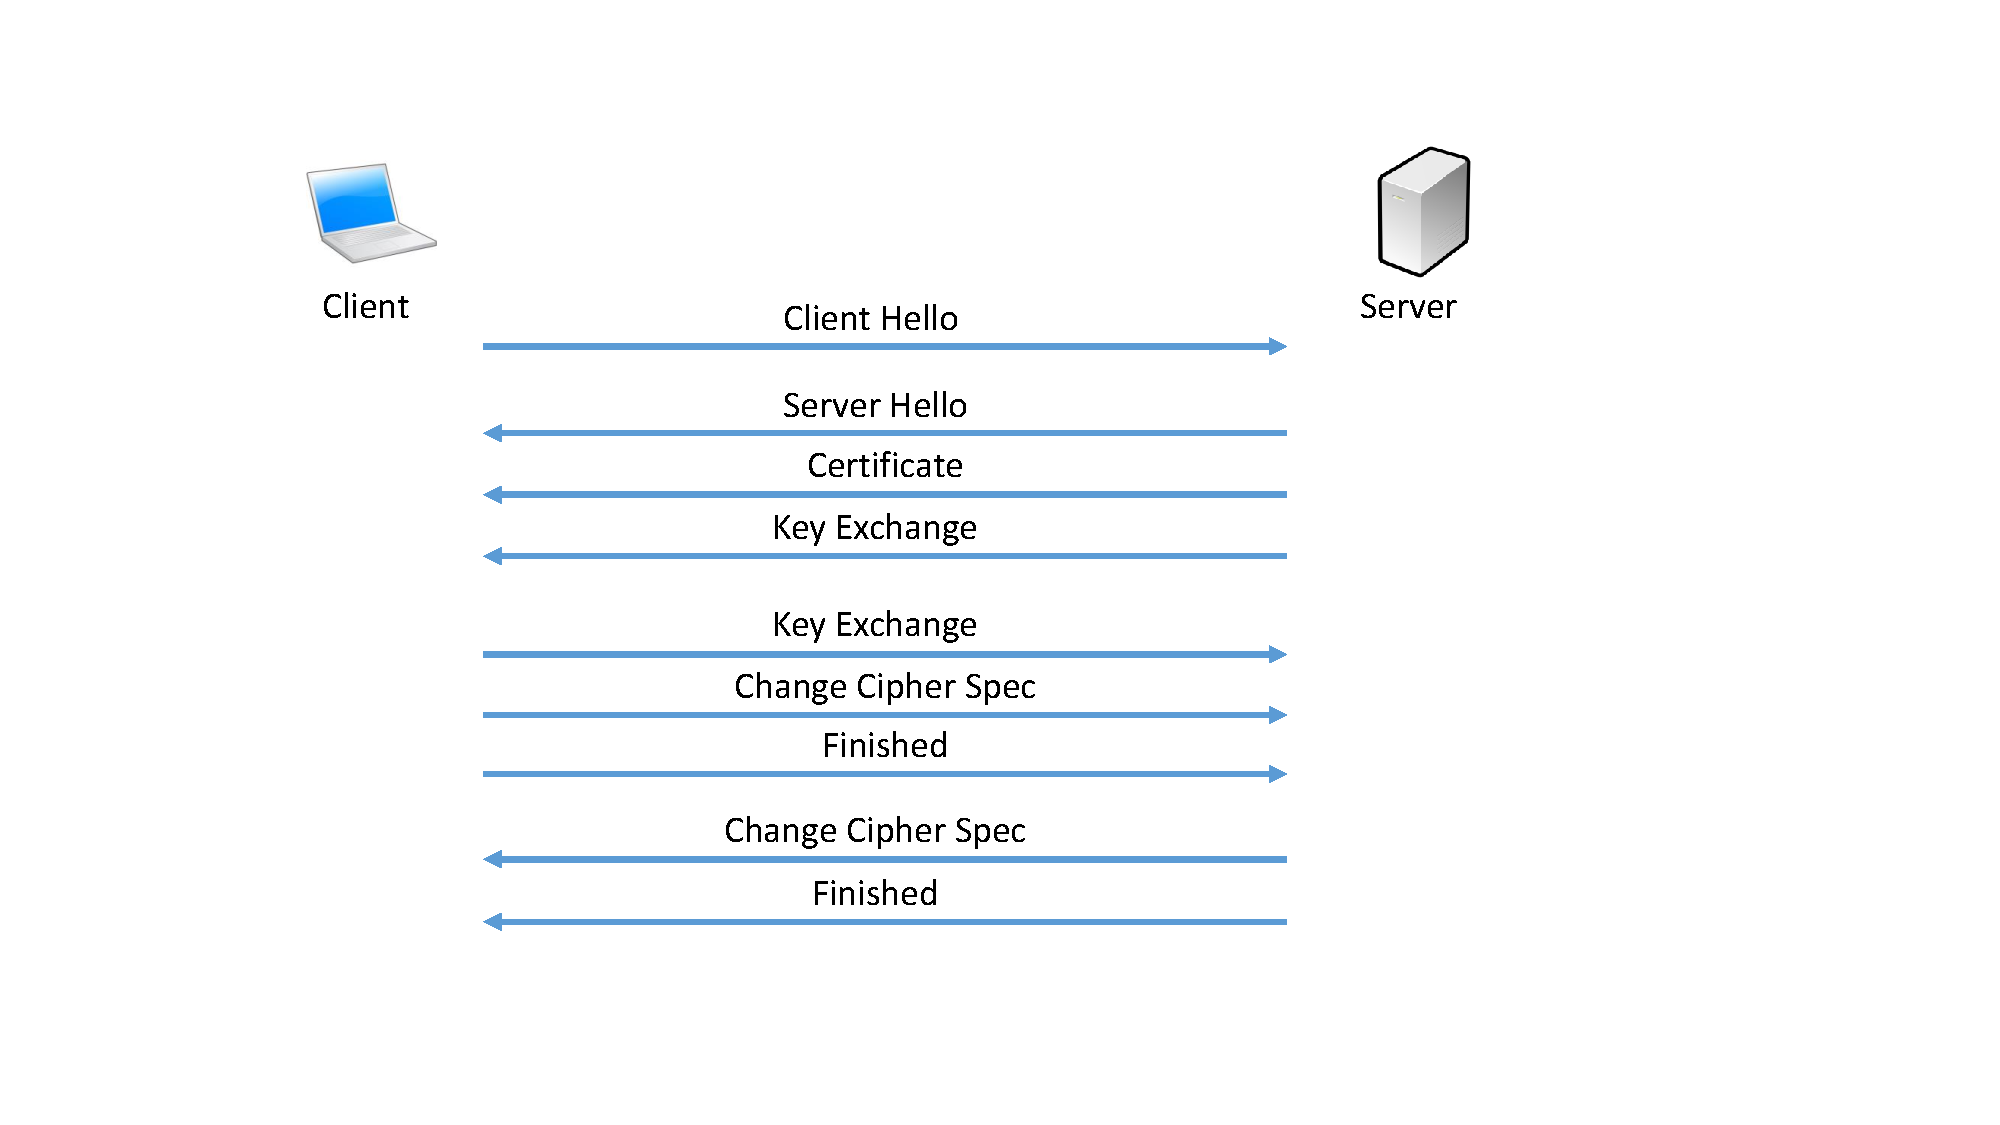
\includegraphics[width=0.9\linewidth,clip]{figures/tls.pdf}
    \caption{\textbf{TLS Handshake}\,---\, %
    The TLS handshake contains several messages sent unencrypted, including the Client Hello.
    This allows us to fingerprint client implementations by the features and parameters they send
    in this initial message.
}
    \label{fig:tls-handshake}
\end{figure}
}

\newcommand{\FigArch}{
\begin{figure*}[ht]
    \centering
    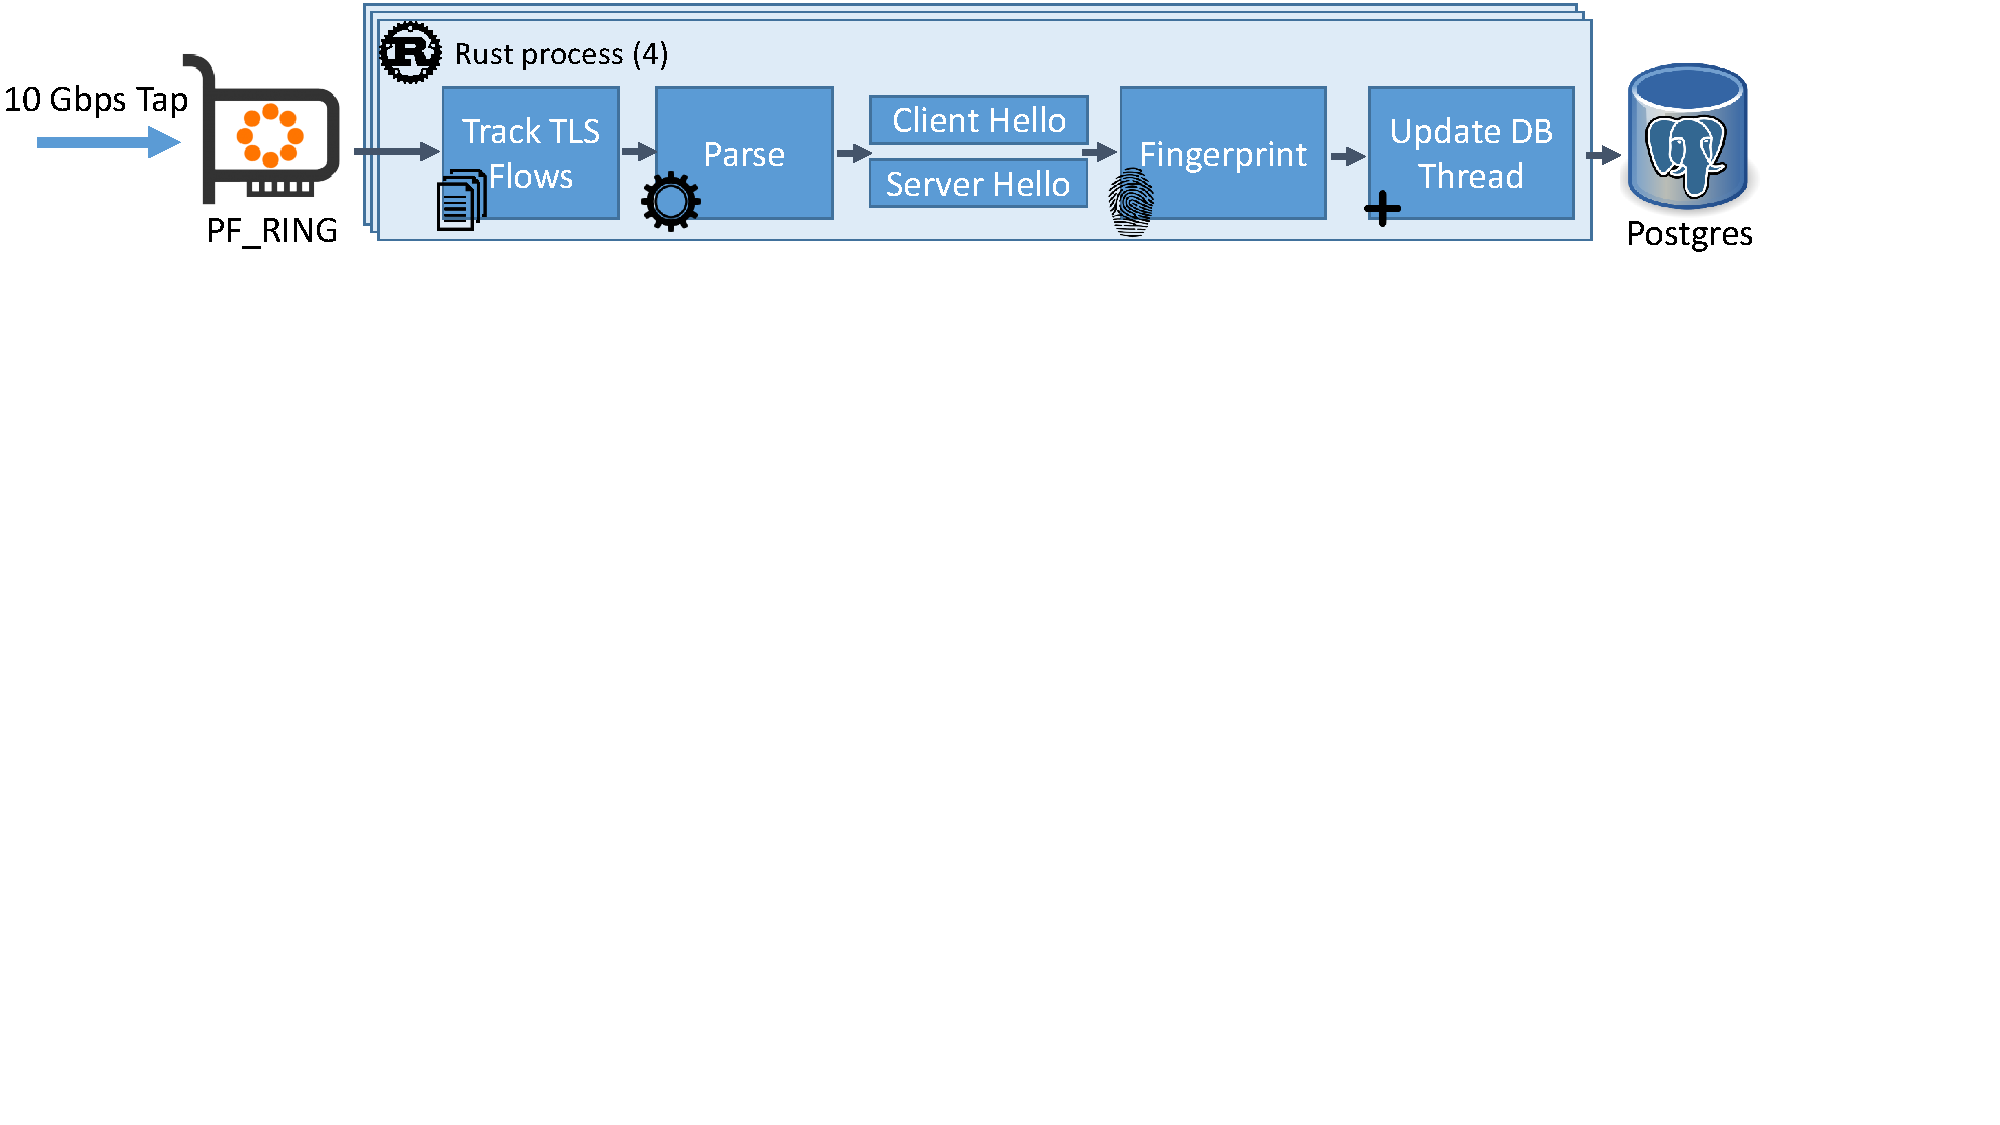
\includegraphics[width=0.9\linewidth,clip]{figures/architecture.pdf}
    \caption{\textbf{Collection Architecture}\,---\, %
    We implemented our 10~Gbps collection infrastructure using PF\_RING and 1400 lines
    of Rust, utilizing 4 processes. TLS client and ServerHello fingerprints and 
    counts
    were aggregated and periodically written to a PostgreSQL database in a separate thread
    to avoid blocking the main packet parsing loop.}
    \label{fig:arch}
\end{figure*}
}

\newcommand{\FigDiff}{
\begin{figure}[ht]
    \centering
    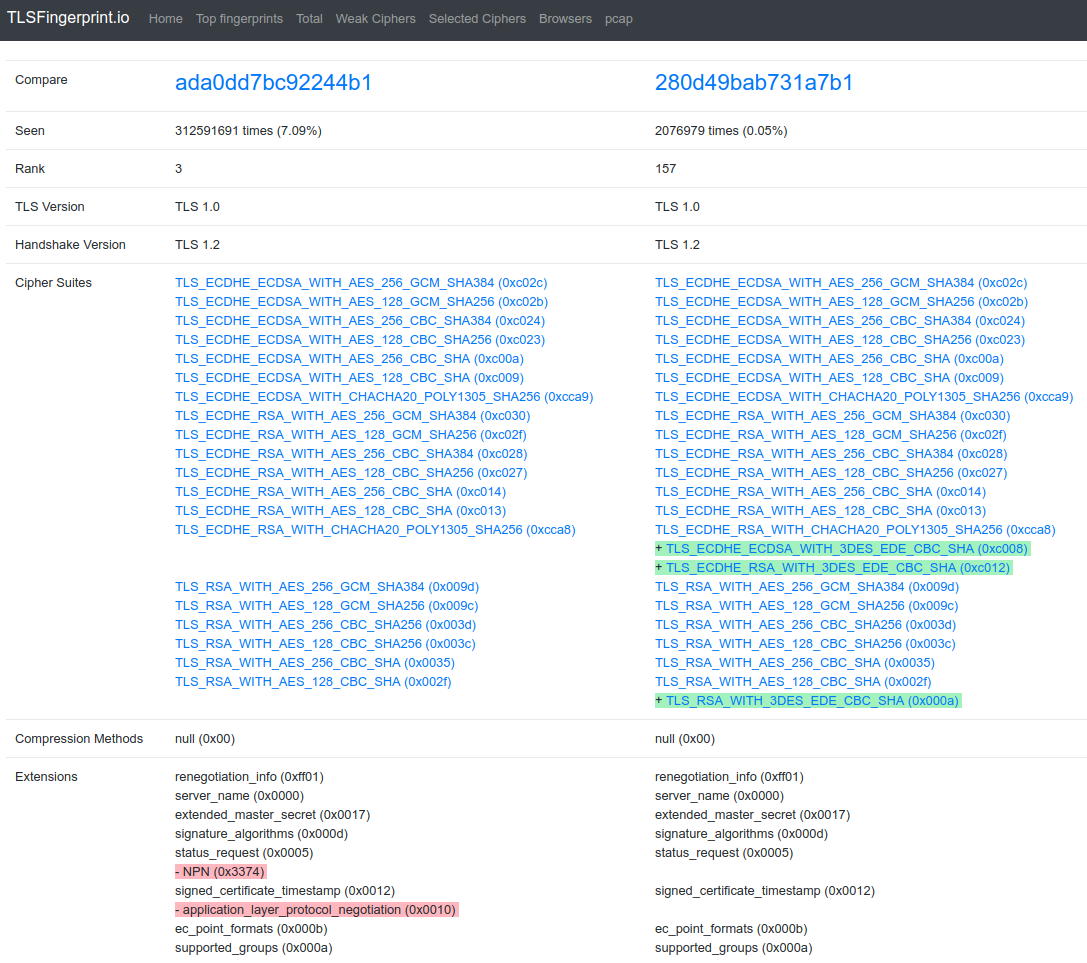
\includegraphics[width=0.9\linewidth,clip]{figures/compare.png}
    \caption{\textbf{Fingerprint comparison}\,---\,Our website supports
            comparing fingerprints and locating similar fingerprints based off
            of a Levenshtein distance over the various ClientHello parts. We
            can then easily show a diff between fingerprints, allowing them to
            be grouped with similar fingerprints generated by the same
    implementation.}
    \label{fig:diff}
\end{figure}
}

\newcommand{\FigTotal}{
\begin{figure}[ht]
    \centering
    \includegraphics[width=0.9\linewidth,clip]{figures/total.pdf}
    \caption{\textbf{Connections observed}\,---\,We collected 9 months of
            TLS connections on our 10~Gbps campus network, observing over 
            11~billion
            connections. Noticeable is
            the diurnal pattern of traffic, as well as a decrease in traffic on weekends
            and holiday breaks.}
    \label{fig:total}
\end{figure}
}

\newcommand{\FigUniqueFingerprints}{
\begin{figure}[ht]
    \centering
    \includegraphics[width=1\linewidth,clip]{figures/tot-uniq.pdf}
    \caption{\textbf{Total Unique Fingerprints}\,---\,The
            number of unique TLS ClientHello fingerprints observed rises
            slowly but steadily over time, reaching over 152,000 by
            May~2018. This rise is
            punctuated by short but rapid increases in the number of unique
            fingerprints, which we determined came
            from a small set of Internet scanners sending seemingly random
    ClientHello messages.}
    \label{fig:tot-uniq}
\end{figure}
}


\newcommand{\FigCDF}{
\begin{figure}[ht]
    \centering
    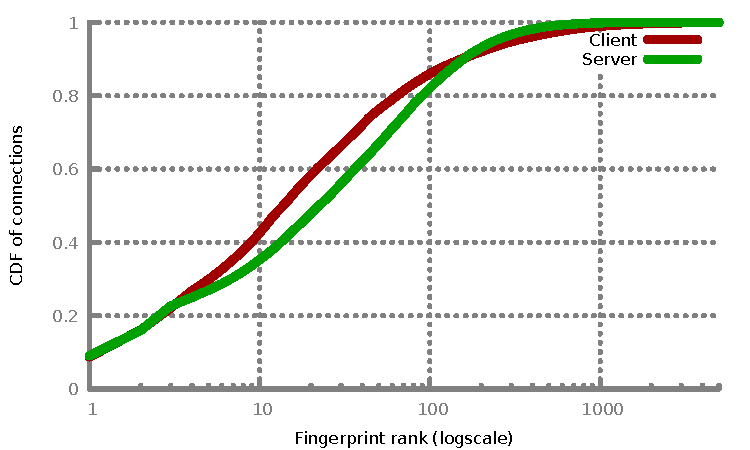
\includegraphics[width=0.9\linewidth,clip]{figures/fingerprints-cdf.pdf}
    \caption{\textbf{CDF of connections per fingerprint}\,---\,
            While we observed over 152,000 ClientHello fingerprints,
            most connections were comprised of a small number of fingerprints:
            over half the connections were of one of the top 12 fingerprints,
            and the top 3000 fingerprints make up 99.9\% of
    connections observed. For servers, only 4,700 fingerprints were observed,
    with half of the connections using one of the top 19 server fingerprints.}
    \label{fig:client-cdf}
\end{figure}
}

\newcommand{\FigServerCDF}{
\begin{figure}[ht]
    \centering
    \includegraphics[width=0.9\linewidth,clip]{figures/sfingerprints-cdf.pdf}
    \caption{\textbf{CDF of server fingerprints}\,---\,
            We observed 3,700 ServerHello fingerprints, and
            most connections were comprised of a small number of fingerprints,
            with top 19 fingerprints being used in over half the connections.
            This CDF is similar to ClientHello CDF, but has a much smaller tail.}
    \label{fig:server-cdf}
\end{figure}
}


\newcommand{\TabInvalid}{
\begin{table}
    \centering
    \scalebox{0.85}{
    \begin{tabular}{ l  c  c }
            \toprule
            & Fingerprints & \% Connections \\
            \hline

            % Updated Aug 7, 2018
            TLS 1.3 draft ciphers &  1002 & 10.626\%    \\
            Legacy ciphers &  82992 & 1.392\%   \\
            GOST ciphers &  95548 & 0.051\% \\
            Outdated SSL ciphers &  106439 & 0.097\%    \\
            Unknown ciphers & 137999 & 0.039\%  \\
            \textbf{Total non-standard ciphers} & \textbf{143060} & \textbf{12.106}\%  \\
            \hline
            TLS 1.3 draft extensions & 715 & 10.626\% \\
            Legacy Extensions & 441 & 0.154\% \\
            Extended Random & 340 & 1.445\% \\
            Unknown extensions & 367 & 0.899\% \\
            \textbf{Total non-standard extensions} & \textbf{1404} & \textbf{11.677}\% \\
            \toprule


        %Invalid ciphers &
            %% Updated: May 7, 2018
            %TLS 1.3 draft ciphers &  776 & 5.236\% \\
            %Legacy ciphers &  62289 & 1.482\% \\
            %GOST ciphers &  70336 & 0.011\% \\
            %Outdated SSL ciphers &  79467 & 0.053\% \\
            %Unknown ciphers & 102175 & 0.002\% \\
            %\textbf{Total non-standard ciphers} & \textbf{106506} & \textbf{6.762\%} \\
            %\hline
            %TLS 1.3 draft extensions & 488 & 5.235\% \\
            %Legacy Extensions & 423 & 0.166\% \\
            %Extended Random & 320 & 1.747\% \\
            %Unknown extensions & 262 & 0.906\% \\
            %\textbf{Total non-standard extensions} & \textbf{1119} & \textbf{6.309\%} \\
            %\toprule


            %Old, from february:
            %TLS 1.3 draft ciphers &  255 & 3.93\%  \\
            %Legacy ciphers &  34200 & 1.65\%   \\
            %GOST ciphers &  37993 & 0.006\% \\
            %Outdated SSL ciphers &  43065 & 0.053\% \\
            %Unknown ciphers & 54920 & 0.002\%   \\
            %\textbf{Total non-standard ciphers} & \textbf{58296} & \textbf{5.63\%}    \\

            %\hline
            %TLS 1.3 draft extensions & 261 & 3.93\% \\
            %Legacy Extensions & 356 & 0.17\%   \\
            %Extended Random & 264 & 3.93\% \\
            %Unknown extensions & 181 & 0.80\% \\
            %\textbf{Total non-standard extensions} & \textbf{775} & \textbf{4.90\%} \\
            %\toprule
    \end{tabular}
    }
    \caption{\textbf{Non-standard parameters}\,---\,
            Breakdown of the number of unique Client Hellos (fingerprints) and
            the share of connections they appear in that send non-standard cipher
            suites or extensions. While TLS~1.3 draft ciphers and extensions are
    the majority, we still find unknown ciphers and extensions in use.}
    \label{tab:invalid}
\end{table}
}

\newcommand{\TabWeak}{
\begin{table}
    \centering
    \begin{tabular}{ l  c  c }
            \toprule
            & Fingerprints & \% Connections \\
            \hline

            % Aug 2018:
            DES & 191459 & 0.90\% \\
            3DES & 236859 & 67.0\% \\
            EXPORT & 194418  & 0.66\% \\
            RC4 & 223900 & 8.19\% \\
            MD5 (Cipher) & 200608 &    7.15\% \\
            \hline
            MD5 (Sigalg) & 4385 & 0.74\% \\
            SHA1 (Sigalg) & 114615 & 97.6\% \\

            TLS\_FALLBACK & 787 & 0.03\% \\


            % May 2018
            %DES & 54727 & 0.92\% \\
            %3DES & 72405 & 61.7\% \\
            %EXPORT & 56543  & 0.67\% \\
            %RC4 & 64075 & 9.13\% \\
            %MD5 (Cipher) & 61050 &    7.92\% \\
 
            %MD5 (Sigalg) & 1686 & 0.70\% \\
            %SHA1 (Sigalg) & 43456 & 97.9\% \\

            %TLS\_FALLBACK & 571 & 0.03\% \\
            \toprule
    \end{tabular}
    \caption{\textbf{Weak ciphers}\,---\, We analyzed the percent of connections
            offering known weak cipher suites. We also include
            \texttt{TLS\_FALLBACK\_SCSV}, which indicates a client that
            is falling back to an earlier version than it supports due to the
            server not supporting the same version.}
    \label{tab:weak}
\end{table}
}

\newcommand{\TabPopularCiphers}{
\begin{table*}[ht]
    \centering
    % view-source:https://tlsfingerprint.io/top-ciphers/
    % Note: excludes fingerprints seen only once...
    \begin{tabular}{ l l c c }
            \toprule
            Rank & Cipher Suite & Fingerprints & \% Connections \\
            \hline
            1  & TLS\_ECDHE\_RSA\_WITH\_AES\_128\_CBC\_SHA & 27798   & 99.1\% \\
            2  & TLS\_ECDHE\_RSA\_WITH\_AES\_256\_CBC\_SHA & 26595   & 98.7\% \\
            3  & TLS\_RSA\_WITH\_AES\_128\_CBC\_SHA &   31014   &  94.4\% \\
            4  & TLS\_RSA\_WITH\_AES\_256\_CBC\_SHA &   30087   &  94.2\% \\
            5  & TLS\_ECDHE\_ECDSA\_WITH\_AES\_128\_GCM\_SHA256 &    27849  &  94.0\% \\
            6  & TLS\_ECDHE\_RSA\_WITH\_AES\_128\_GCM\_SHA256 &  24642   &  92.6\% \\
            7  & TLS\_ECDHE\_ECDSA\_WITH\_AES\_256\_GCM\_SHA384 &    25643 &  92.5\% \\
            8  & TLS\_ECDHE\_RSA\_WITH\_AES\_256\_GCM\_SHA384 &  21891   &  91.1\% \\
            9  & TLS\_RSA\_WITH\_AES\_128\_GCM\_SHA256 &    26130   &  84.6\% \\
            10 & TLS\_RSA\_WITH\_AES\_256\_GCM\_SHA384 &    23635   &  83.2\% \\
            \toprule
    \end{tabular}
    \caption{\textbf{Popular Cipher Suites}\,---\, Top ten popular cipher suites offered by clients,
                weighted by connections. Small handful of cipher suites appear to be
                supported by the vast majority of clients in use.}
    \label{tab:popularciphers}
\end{table*}
}

\newcommand{\TabTopFingerprints}{
\begin{table}[ht]
    \centering
    % view-source:https://tlsfingerprint.io/top-ciphers/
    % Note: excludes fingerprints seen only once...
        \textbf{August 2018}
    \begin{tabular}{ r l c }
            \toprule
            Rank & Client & \% Connections \\
            \hline
            1  & Chrome 65-68 & 16.51\%   \\  % 177
            2  & iOS 11/macOS 10.13 Safari & 5.95\%        \\  % 77
            3  & MS Office 2016 (including Outlook) &  5.34\% \\ % 338
            4  & Chrome 65-68 (with padding) &  4.62\% \\   % 177
            5  & Edge 15-18, IE 11 &  4.05\% \\    % 338
            6  & Firefox 59-61 (with padding) &  3.62\% \\  % 48
            7  & Safari 11.1 on Mac OS X &  2.82\% \\   % 77
            8  & iOS 10/macOS 10.12 Safari & 2.49\% \\ % 51
            9  & iOS 11/macOS 10.13 Safari (with padding) & 2.42\% \\ % 77
            10 & Firefox 59-61 & 2.22\% \\ % 48
            \toprule
    \end{tabular}
        \\
        \textbf{December 2018} \\
    \begin{tabular}{ r l c }
            \toprule
            Rank & Client & \% Connections \\
            \hline
            1    & Chrome 70 (with padding) & 8.49\% \\
            2    & iOS 12/macOS 10.14 Safari & 7.55\% \\
            3    & iOS 12/macOS 10.14 Safari (without ALPN) & 4.15\% \\
            4    & Chrome 70 & 4.10\% \\
            5    & iOS 12/macOS 10.14 Safari (with padding) & 4.09\% \\
            6    & Edge 15-18, IE 11 & 3.27\% \\
            7    & MS Office 2016 (including Outlook) & 3.01\% \\ 
            8    & iOS 10/macOS 10.12 Safari & 2.72\% \\
            9    & iOS 11/macOS 10.13 Safari & 2.68\% \\
            10   & Chrome 71 (with padding) & 2.48\% \\ % released Dec 4th
            \toprule
    \end{tabular}
    \caption{\textbf{Top 10 Implementations.}\,---\, Most frequently seen fingerprints in our
        dataset and the implementations that generate them, for a week in August and December~2018.
        Despite being only 4 months apart,
        top 10 fingerprints changed substantially, as
        new browser releases quickly take the place of older versions.}

        %These implementations are responsible for generating just over half the connections we see.
    %Rank and amount of connections are for one week of measurements in early August 2018.
    %Fingerprints with and without padding are otherwise identical: the padding extension is commonly
    %added by TLS stacks to work around bugs in deployed middleboxes.}
    \label{tab:toptenfingerprints}
\end{table}
}

\newcommand{\TabTopFingerprintsDecember}{
\begin{table}[ht]
    \centering
    % view-source:https://tlsfingerprint.io/top-ciphers/
    % Note: excludes fingerprints seen only once...
    \begin{tabular}{ r l c }
            \toprule
            Rank & Client & \% Connections \\
            \hline
            1    & Chrome 70 with padding & 8.49\% \\
            2    & iOS 12/macOS 10.14 Safari & 7.55\% \\
            3    & iOS 12/macOS 10.14 Safari without ALPN & 4.15\% \\
            4    & Chrome 70 & 4.10\% \\
            5    & iOS 12/macOS 10.14 Safari with padding & 4.09\% \\
            6    & Edge 15-18, IE 10 on Windows 10 & 3.27\% \\
            7    & MS Office 2016 & 3.01\% \\ 
            8    & iOS 10/macOS 10.12 Safari & 2.72\% \\
            9    & iOS 11/macOS 10.13 Safari & 2.68\% \\
            10   & Chrome 71 with padding & 2.48\% \\ % released Dec 4th
            \toprule
    \end{tabular}
    \caption{\textbf{Top 10 Implementations. December, 2018}\,---\, Most frequently seen fingerprints in our
        dataset and the implementations that generate them.
    Rank and amount of connections are for one week of measurements in between December 6th and 13th 2018:
    Chrome 71 was released on December 4th and is gradually replacing Chrome 70.
    Note that Chrome started to generate padded version more often than non-padded:
    padding is included when ClientHello is between 256 and 512 bytes long
    to work around bugs in deployed middleboxes,
    and addition of new TLS 1.3 extensions with new data made ClientHellos
    go over 256 bytes more often.
    }
    \label{tab:toptenfingerprints}
\end{table}
}

\newcommand{\TabSelectedCiphers}{
\begin{table*}[ht]
    \centering
    % view-source:https://tlsfingerprint.io/server-ciphers
    \tabcolsep=0.11cm
    \scalebox{0.9}{
    \begin{tabular}{l c c c }
            \toprule
        Cipher Suite & Client Fingerprints & Server Fingerprints & \% Connections \\
            \hline

            TLS\_ECDHE\_RSA\_WITH\_AES\_128\_GCM\_SHA256 & 5137 & 438 & 50.71 \\

            TLS\_ECDHE\_RSA\_WITH\_AES\_256\_GCM\_SHA384 & 3054 & 268 & 19.29 \\

            TLS\_ECDHE\_ECDSA\_WITH\_AES\_128\_GCM\_SHA256 & 1656 & 264 & 13.30 \\

            TLS\_ECDHE\_ECDSA\_WITH\_AES\_256\_GCM\_SHA384 & 765 & 115 & 2.45 \\

            TLS\_RSA\_WITH\_AES\_256\_CBC\_SHA & 1300 & 123 & 1.60 \\

            TLS\_RSA\_WITH\_AES\_256\_CBC\_SHA256 & 2711 & 45 & 1.56 \\

            TLS\_RSA\_WITH\_AES\_128\_CBC\_SHA & 2688 & 134 & 1.49 \\

            TLS\_ECDHE\_RSA\_WITH\_CHACHA20\_POLY1305\_SHA256 & 333 & 170 & 1.38 \\

            TLS\_RSA\_WITH\_AES\_256\_GCM\_SHA384 & 855 & 56 & 1.38 \\

            TLS\_ECDHE\_RSA\_WITH\_AES\_256\_CBC\_SHA384 & 1023 & 121 & 1.31 \\

            % Top 10: 94.40% of connections total
            \toprule
    \end{tabular}
    }
    \caption{\textbf{Server Hello Selected Ciphers}\,---\,The top ten most common ciphers selected accounted for
            over 94\% of connections with all connections choosing one of only 47 cipher suites,
            showing significantly less server diversity than client fingerprints, which had over 6600 unique sets
            of cipher suites sent in 21,000 ClientHello fingerprints seen more 
            than once.}
    \label{tab:selected}
\end{table*}
}


\newcommand{\TabSelectedALPN}{
\begin{table}
    % From https://tlsfingerprint.io/alpn
    \centering
    \tabcolsep=0.11cm
    \scalebox{0.9} {
    \begin{tabular}{r c c}
            \toprule

            % May 2018
            ALPN & Fingerprints & \% Connections \\
            \hline
            \emph{None} & 156247 & 58.4\% \\
            h2 & 22562 & 22.0\% \\
            http/1.1 & 36292 & 19.3\% \\
            apns-pack-v1:4096:4096 & 3 & 0.2\% \\
            spdy/3.1 & 1313 & 0.1\% \\


            % February 2018:
            %Selected ALPN & Fingerprints & \% Connections \\
            %\hline
            %\emph{None} & 72681 & 58.38\% \\
            %    h2 & 13101 & 22.36\% \\
            %    http/1.1 & 21040 & 18.92\% \\
            %    spdy/3.1 & 902 & 0.18\% \\
            %    apns-pack-v1:4096:4096 & 3 & 0.16\% \\
            \toprule
    \end{tabular}
    }
    \caption{\textbf{Selected ALPN}\,---\, Top five most commonly selected ALPN. HTTP/2 outranks
            explicit HTTP/1.1 support, though likely the majority of connections that
            provided no ALPN (58\%) defaulted to HTTP/1.1. Despite only having 3 distinct fingerprints,
            Apple's push notification service (APNS) accounts for 0.16\% of all connections.
    }
    \label{tab:selectedALPN}
\end{table}
}


\newcommand{\TabTools}{
	\begin{table}
		\centering
		\tabcolsep=0.11cm
		\scalebox{0.9} {
			\begin{tabular}{l r l l}
				\toprule
                    Tool & Version/Date & Rank [all time] & \% Connections \\
				\hline
                    \textbf{Psiphon} & Jan 2018 & 1 & 8.76\% \\
                    & & 9 & 2.42\% \\
                    & & 62 & 0.25\% \\
                    & & 198 & \textcolor{red}{0.04\%} \\
                    & & 203 & \textcolor{red}{0.04\%} \\
                    & & 500 & \textcolor{red}{0.01\%} \\
                    & & 2190 & \textcolor{red}{0.0002\%} \\
                    & & 14397 & \textcolor{red}{0.0000\%} \\ % < 0.0001%
                    & & 16814 & \textcolor{red}{0.0000\%} \\ % < 0.0001
%\hline
                    \textbf{Outline} & May 2018 & 1 & 8.76\% \\
%\hline
                    \textbf{meek} & TBB 7.5 & 42 & 0.50\% \\
%\hline
                    \textbf{Snowflake} & April 2018 & 1378 & \textcolor{red}{0.0008\%} \\
%\hline
                    \textbf{Lantern} & 4.6.13 & 1867 & \textcolor{red}{0.0003\%} \\
%\hline
                    \textbf{TapDance} & May 2018 & random & - \\
%\hline
                    \textbf{Signal} & 4.19.3 & 11468 & \textcolor{red}{0.0000\%} \\
                    &   & 12982 & \textcolor{red}{0.0000\%} \\
				\toprule
			\end{tabular}
		}
		\caption{\textbf{Tool Fingerprintability}\,---\, Summary of all TLS
		fingerprints generated by censorship circumvention tools and their
            rank and percent of connections seen in our dataset as of early August 2018.
            Highlighted in red are fingerprints seen in relatively few ($<$ 0.1\%)
            connections, putting them at risk of blocking by a censor.
		}
		\label{tab:tools}
	\end{table}
}

\newcommand{\TabPopularALPN}{
\begin{table}
    % From https://tlsfingerprint.io/alpn
    \centering
    \tabcolsep=0.11cm
    \scalebox{0.9} {
    \begin{tabular}{r c c}
            \toprule


        % Updated Aug 7, 2018
        ALPN & Fingerprints & \% Connections \\
        \hline
                http/1.1 & 8078 & 70.3\% \\
                h2 & 5200 & 64.1\% \\
                spdy/3.1 & 2421 & 23.2\% \\
                spdy/3 & 1006 & 22.5\% \\
                h2-14 & 755 & 19.9\% \\
                h2-15 & 460 & 19.9\% \\
                h2-16 & 472 & 19.9\% \\
                h2-fb & 99 & 0.3\% \\
                apns-pack-v1 & 2 & 0.1\% \\
                apns-security-v3 & 2 & 0.1\% \\

        % May 2018
        %http/1.1 & 7032 & 70.8\% \\
        %h2 & 4534 & 64.6\% \\
        %spdy/3.1 & 2219 & 25.0\% \\
        %spdy/3 & 901 & 24.3\% \\
        %h2-14 & 664 & 21.5\% \\
        %h2-15 & 389 & 21.4\% \\
        %h2-16 & 399 & 21.4\% \\
        %h2-fb & 85 & 0.3\% \\
        %apns-pack-v1 & 2 & 0.1\% \\
        %apns-security-v3 & 2 & 0.1\% \\


            % February 2018:
            %ALPN & Fingerprints & \% Connections \\
            %    \hline
            %        http/1.1 & 5807 & 70.7\% \\
            %        h2 & 3748 & 64.4\% \\
            %        spdy/3.1 & 1971 & 26.0\% \\
            %        spdy/3 & 776 & 25.2\% \\
            %        h2-14 & 549 & 22.2\% \\
            %        h2-15 & 298 & 22.1\% \\
            %        h2-16 & 310 & 22.1\% \\
            %        h2-fb & 53 & 0.3\% \\
            %        apns-pack-v1 & 2 & 0.1\% \\
            %        apns-security-v3 & 2 & 0.1\% \\
            \toprule
    \end{tabular}
    }
    \caption{\textbf{Popular ALPN}\,---\, Top most commonly supported ALPNs. In total, there
            were 526 unique ALPN values sent by clients, though the vast majority were invalid random values.
            Prominent in this data is support for HTTP/2 (h2) and its draft versions,
            Google's \texttt{spdy} protocol, and Apple's Push Notification Service (APNS) protocol.
    }
    \label{tab:popularALPN}
\end{table}
}

\newcommand{\FigTopNoSNI}{
    \begin{figure}[ht]
        \centering
    \includegraphics[width=0.9\linewidth,clip]{figures/sniless-cdf.pdf}
    \caption{\textbf{CDF of connections sending no SNI}\,---\, %
        We observed 1.4\% of connections did not send the server name indication (SNI)
        extension, with the majority coming from just 10 fingerprints. This suggests a censor
        could easily block circumvention tools that do not send SNIs, with either a small
        amount of collateral overblocking or minimal whitelisted exceptions.}
    \label{fig:sniless-cdf}
    \end{figure}
}

\newcommand{\TabTopNoSNI}{
	\begin{table}[ht]
		% From https://tlsfingerprint.io/alpn
		\centering
		\tabcolsep=0.11cm
		\scalebox{0.9} {
			\begin{tabular}{r c}
				\toprule
				Rank & Connections [all time] \\ %& Rank [all time] & Rank 
				%[25 April 
				%- 2 May 2018] \\
				\hline
1 & 0.1956 \% \\  %& 68 & 77 \\
2 & 0.0857 \% \\  %& 111 & 137 \\
3 & 0.0745 \% \\  %& 125 & 314 \\
4 & 0.0560 \% \\  %& 140 & - \\
5 & 0.0540 \% \\  %& 143 & 152 \\
6 & 0.0499 \% \\  %& 149 & 153 \\
7 & 0.0478 \% \\  %& 160 & 143 \\
8 & 0.0476 \% \\  %& 163 & 164 \\
9 & 0.0471 \% \\  %& 164 & 227 \\
10 & 0.0450 \%\\  % & 167 & 948 \\

%8577568175451810252  
%-6423993798557871268 
%1380591653976699571  
%-2791419216777605277 
%-5231413793168069546 
%417772208000436940   
%502795999810062699   
%3080265117687502513  
%-4261455803793459001 
%-3124589779202159765 
%-2022210942072690627 & 0.0438 \% & 169 & 161 \\
				\toprule
			\end{tabular}
		}
		\caption{\textbf{Top fingerprints that lack SNI}\,---\,
            TODO: this would be better as a CDF...
			Top ten popular fingerprints, that lack SNI,
			weighted by connections.
            %and their relative popularity as of May 2, 2018.
            In total, only TK\% of connections sent no SNI, suggesting that it
            would not cause sigificant collateral damage for a censor to block
            TLS connections that do not send this extension.
			%that they are used by bots, including top 1, 3 and 4 SNI-less
			%fingerprints of all time.
		}
		\label{tab:topNoSNI}
	\end{table}
}

\newcommand{\TabExtensions}{
    \begin{table}[ht]
        \centering
            \begin{tabular}{r l}
                \toprule
                Extension & Conns \\
                \hline
                    \textbf{supported\_groups} & 99.4\% \\
                    server\_name & 99.3\% \\
                    \textbf{signature\_algorithms} & 97.8\% \\
                    \textbf{ec\_point\_formats} & 96.9\% \\
                    extended\_master\_secret & 86.8\% \\
                    status\_request & 85.7\% \\
                    renegotiation\_info & 81.9\% \\
                    \textbf{ALPN} & 71.9\% \\
                    signed\_certificate\_timestamp & 66.9\% \\
                    SessionTicket & 56.0\% \\
                    padding & 32.3\% \\
                \toprule
            \end{tabular}
            \begin{tabular}{r l}
                \toprule
                Extension & Conns \\
                \hline
                    GREASE & 30.2\% \\
                    \textbf{psk\_key\_exchange\_modes}* & 28.7\% \\
                    \textbf{supported\_versions}* & 28.7\% \\
                    \textbf{key\_share}* & 28.6\% \\
                    NPN & 27.3\% \\
                    \textbf{compressed\_certificate}* & 24.8\% \\
                    ChannelID & 20.5\% \\
                    heartbeat & 5.0\% \\
                    token\_binding & 3.9\% \\
                    pre\_shared\_key* & 3.1\% \\
                    \textbf{record\_size\_limit} & 2.5\% \\
                \toprule
                \end{tabular}
            \caption{\textbf{Top Extensions}\,---\,
            While we include the presence and order of all extensions in our fingerprint,
            \textbf{Bold} denotes extensions whose data we additionally parse and include in our fingerprint;
            * marks extensions new in TLS~1.3.
            %Data shown for a week between December 5th and 12th, 2018.
            }
            \label{tab:extensions}
        \end{table}
}
